\chapter{Introduction}
\label{sec:introduction}
\begin{itemize}
\item Metaversion is a virtual universe that integrates VR, AR, and the Internet, providing a shared, immersive, and often three-dimensional space for online interaction and presence.
\item The Metaverse is a virtual world where users interact with digital avatars that reflect their identity and physical characteristics.
\item Metaversion, incorporating virtual offices, classrooms, and training environments, offers new opportunities for learning, skill development, and remote collaboration in both entertainment and education.
\end{itemize}
\section{History of the Metaverse}
Metaversion, also known as collective virtual shared space or virtual reality space, has a rich history rooted in science fiction, technology, and online communities. Here's a brief overview of the meta version's history:
\subsection{1970 - Sci-Fi Origins:}
Neal Stephenson's 1992 novel "Snow Crash" popularized the concept of metaversion, a virtual reality space where users interact as avatars, serving as a conceptual basis for later developments.
\subsection{Early Virtual Worlds:}
In the late 1970s and 1980s, MUDs and MOOs were online environments that enabled multiple users to interact in text-based virtual worlds, paving the way for modern online communities.
\subsection{1990 - Emergence of 3D Virtual Worlds:}
In the 1990s, 3D virtual worlds like Second Life emerged, enabling users to create avatars, socialize, and build virtual environments, paving the way for immersive metaverse experiences.
\subsection{2000 - Online Games and Social Media:}
Online interactions and communities are transforming MMOs like World of Warcraft and social media platforms like Facebook and Twitter, fostering connected digital spaces.
\subsection{2010 - VR and AR:}
Virtual and augmented reality technologies, like Oculus Rift and HTC Vive, are revolutionizing metaversion by providing immersive virtual spaces through smartphones and AR glasses.

\subsection{Current developments:}
As of September 2021, companies are developing meta-related technologies like virtual reality, augmented reality, blockchain, and decentralized platforms, using NFTs to represent digital assets within the metaverse.
\section{The Future of the Metaverse}
Metaversion, a future of immersive virtual and augmented reality experiences, blockchain-based asset ownership, and economic opportunities, is expected to revolutionize various sectors, redefining social dynamics, raising concerns about privacy, security, regulation, and environmental sustainability.
\begin{figure}[h]
    \centering
    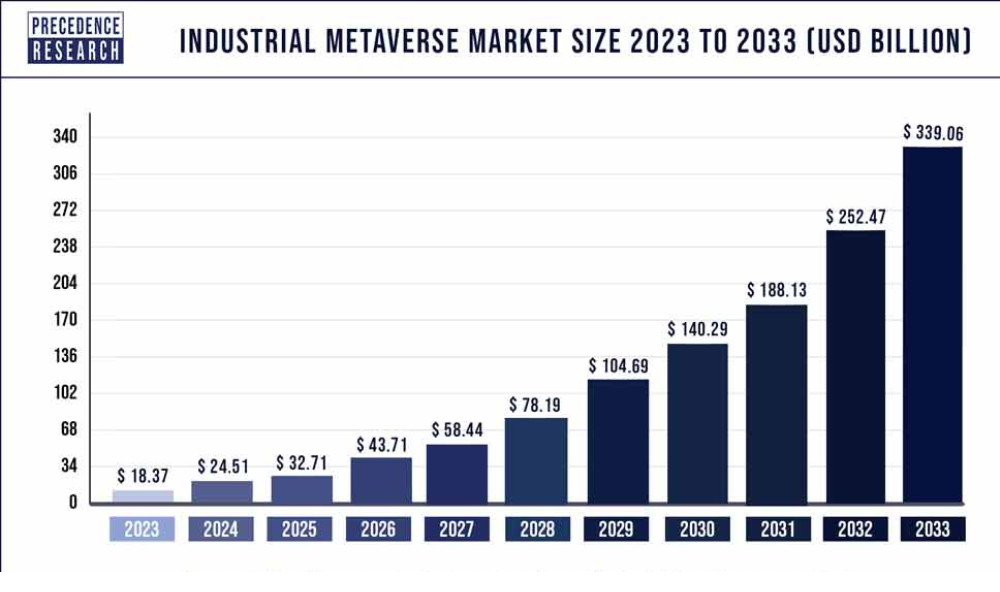
\includegraphics[width=0.8\textwidth, height=0.35\textheight]{Images/industrial-metaverse-market-size.png}
    \caption{Future of Metaverse}
    \label{fig:Future of Metaverse}\cite{metaverse-market}
\end{figure}
\section{How Metaverse Would Excel}
The success of the metaverse will be influenced by several key factors:\\
\textbf{Technology Advances:}\\ The metaverse's success relies on advancements in technologies like VR, AR, AI, and high-speed internet connectivity, along with enhanced hardware and software for immersive virtual experiences.\\
\textbf{User Adoption:}\\ The metaverse's success relies on a critical mass of active users, with user-friendly interfaces and accessibility playing a crucial role in attracting a diverse user base.\\
\textbf{Content and Creativity:}\\ The Metaverse requires a diverse range of engaging content, experiences, and activities, including virtual worlds, games, social spaces, art, and educational content, for easy creation and sharing.\\
\textbf{Interoperability and standards:}\\ Open standards and protocols for the metaverse are crucial for creating a seamless, accessible environment by facilitating interoperability between virtual worlds and platforms.\\
\textbf{Security and Privacy:}\\ Users must rely on metaverse for their personal data and transactions, requiring robust security measures, data protection, and privacy controls to prevent abuse, fraud, and unauthorized access.\\
\textbf{Economic Viability:}\\ Metaversion necessitates a sustainable economy, attracting users and content creators through virtual real estate, digital currencies, and employment opportunities, utilizing blockchain technology and NFTs.\\
\textbf{Regulation and governance:}\\ Governments and regulators will need to create clear guidelines and legal frameworks for meta